\documentclass[aspectratio=169,11pt,hyperref={colorlinks=true}]{beamer}
\usetheme{boxes}
\setbeamertemplate{navigation symbols}{}
\definecolor{openstack}{RGB}{149,0,4}
\setbeamercolor{titlelike}{fg=openstack}
\setbeamercolor{structure}{fg=openstack}
\hypersetup{colorlinks,urlcolor=openstack}
\setbeamertemplate{footline}[frame number]
% Inserting graphics
\usepackage{graphicx}
% Side-by-side figures, etc
\usepackage{subfigure}
% Code snippits
\usepackage{listings}
% Color stuff
\usepackage{color}
\usepackage{amsmath}
\usepackage{tikz}
\usepackage{tipa}
\newcommand\RBox[1]{%
  \tikz\node[draw,rounded corners,align=center,] {#1};%
}
\usepackage{hyperref}
%\usecolortheme{buzz}
%\usecolortheme{wolverine}
%\usetheme{Boadilla}
\usepackage[T1]{fontenc}

\definecolor{mygreen}{rgb}{0,0.6,0}
\definecolor{mygray}{rgb}{0.5,0.5,0.5}
\definecolor{mymauve}{rgb}{0.58,0,0.82}

\lstset{ %
  backgroundcolor=\color{white},   % choose the background color; you must add \usepackage{color} or \usepackage{xcolor}
  breakatwhitespace=false,         % sets if automatic breaks should only happen at whitespace
  breaklines=true,                 % sets automatic line breaking
  captionpos=b,                    % sets the caption-position to bottom
  commentstyle=\color{openstack},  % comment style
  extendedchars=true,              % lets you use non-ASCII characters; for 8-bits encodings only, does not work with UTF-8
  keepspaces=true,                 % keeps spaces in text, useful for keeping indentation of code (possibly needs columns=flexible)
  keywordstyle=\color{blue},       % keyword style
  otherkeywords={*,...},           % if you want to add more keywords to the set
  numbersep=5pt,                   % how far the line-numbers are from the code
  numberstyle=\tiny\color{mygray}, % the style that is used for the line-numbers
  rulecolor=\color{black},         % if not set, the frame-color may be changed on line-breaks within not-black text (e.g. comments (green here))
  showspaces=false,                % show spaces everywhere adding particular underscores; it overrides 'showstringspaces'
  showstringspaces=false,          % underline spaces within strings only
  showtabs=false,                  % show tabs within strings adding particular underscores
  stringstyle=\color{openstack},   % string literal style
}

\setbeamerfont{caption}{series=\normalfont,size=\fontsize{6}{8}}
\setbeamertemplate{caption}{\raggedright\insertcaption\par}

\setlength{\abovecaptionskip}{0pt}
\setlength{\floatsep}{0pt}

\AtBeginSection[]{
  \frame<beamer>{
      \centering \huge \insertsectionhead \par%
      \includegraphics[width=0.3\textwidth]{OpenStack_Project_QA_horizontal.png}
  }
}

\author[Andrea Frittoli]{%
    \texorpdfstring{
        \begin{columns}
            \column{.45\linewidth}
            \centering
            Andrea Frittoli\\
            \href{mailto:andrea.frittoli@gmail.com}{andrea.frittoli@gmail.com}\\
            \texttt{andreaf on Freenode}
        \end{columns}
   }
   {Andrea Frittoli}
}
\date{Nov 7, 2017}

\title[QA Project Update - Sydney, Nov 2017
\hspace{2em}\insertframenumber/\inserttotalframenumber]{OpenStack QA Project Overview and Update}

\begin{document}

{
\setbeamertemplate{background canvas}{
\includegraphics[width=\paperwidth,height=\paperheight]{background_title.png}}
\setbeamertemplate{footline}{}
\begin{frame}[noframenumbering]
    \setbeamercolor{titlelike}{fg=white}
    \setbeamercolor{structure}{fg=white}
    \setbeamercolor{normal text}{fg=white}
    \hypersetup{colorlinks,urlcolor=white}
    \setbeamercolor{author}{fg=white}
    \setbeamercolor{date}{fg=white}
    \setbeamercolor{background}{bg=openstack}
    \titlepage{}
    \centering
    \href{https://github.com/afrittoli/qa-project-update}{https://github.com/afrittoli/qa-project-update}
\end{frame}
}

\begin{frame}[c]
    \frametitle{}
    \begin{center}
        
\includegraphics[width=1.0\textwidth]{OpenStack_Project_QA_vertical.png}
    \end{center}
\end{frame}

\section{OpenStack QA Overview}
\begin{frame}
    \frametitle{What is OpenStack QA?}
    \begin{itemize}
     \item Official Mission Statement:\\
         \textit{Develop, maintain, and initiate tools and plans to ensure
the upstream stability and quality of OpenStack, and its release readiness at
any point during the release cycle.}
    \end{itemize}
\end{frame}

\begin{frame}
    \frametitle{Current QA Projects}
    \begin{columns}
    \begin{column}{0.5\textwidth}
    \begin{itemize}
        \item{devstack}
        \item{devstack-tools}
        \item{tempest}
        \item{patrole}
        \item{grenade}
        \item{hacking}
        \item{bashate}
        \item{eslint-config-openstack}
    \end{itemize}
    \end{column}
    \begin{column}{0.5\textwidth}
    \begin{itemize}
        \item{openstack-health dashboard}
        \item{stackviz}
        \item{os-testr}
        \item{devstack-plugin-cookiecutter}
        \item{tempest-plugin-cookiecutter}
        \item{os-performance-tools}
        \item{devstack-plugin-ceph}
        \item{devstack-vagrant}
    \end{itemize}
    \end{column}
    \end{columns}
\end{frame}

\begin{frame}
    \frametitle{Things we do}
    \begin{columns}
    \begin{column}{0.5\textwidth}
    \begin{itemize}
        \item{Community driven approach to QA}
        \item{Serve the OpenStack community}
        \item{Drive testing best practices}
        \item{Maintain test tools and frameworks}
        \item{Keep the gate running smoothly}
        \item{Support interoperability testing efforts}
    \end{itemize}
    \end{column}
    \begin{column}{0.5\textwidth}
        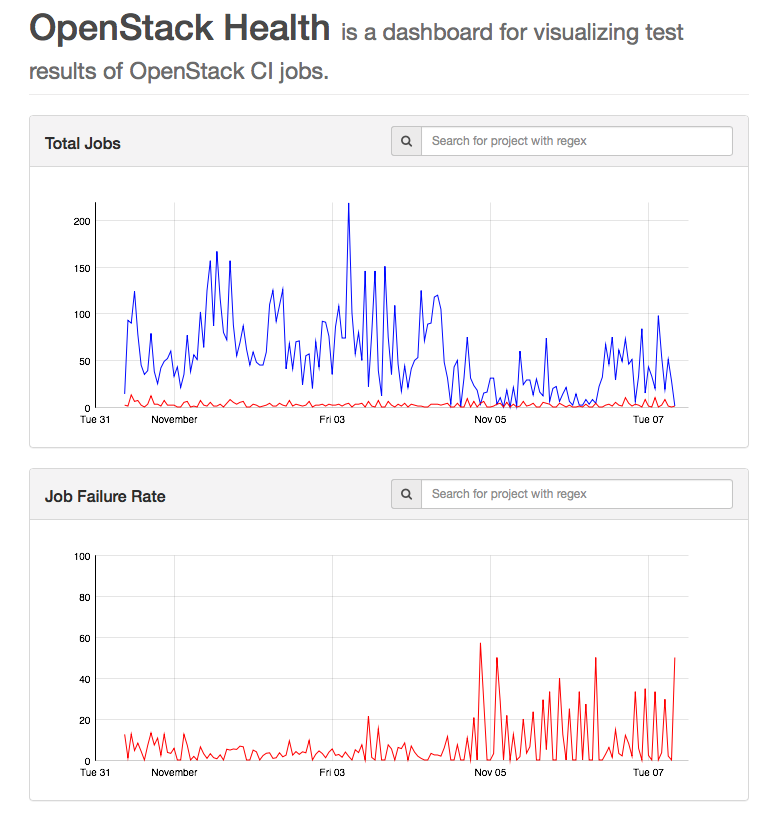
\includegraphics[width=1.0\textwidth]{openstack-health.png}
    \end{column}
    \end{columns}
\end{frame}

\section{Updates from Queens}
\begin{frame}
    \frametitle{Tempest}
    \begin{itemize}
        \item{Several Tempest APIs are now stable}
        \begin{itemize}
            \item{Credential providers}
            \item{Service clients}
            \item{Test base class (for plugins)}
        \end{itemize}
        \item{Scenario code cleanup}
    \end{itemize}
\end{frame}

\begin{frame}
    \frametitle{Tempest Plugins Goal}
    \begin{itemize}
        \item{https://governance.openstack.org/tc/goals/queens/split-tempest-plugins.html}
        \item{https://docs.openstack.org/tempest/latest/plugin-registry.html}
    \end{itemize}
\end{frame}

\begin{frame}
    \frametitle{Test Runners}
    \begin{itemize}
        \item{stestr: http://stestr.readthedocs.io/en/latest/}
        \item{os-testr}
        \item{tempest}
    \end{itemize}
\end{frame}

\begin{frame}
    \frametitle{ZuulV3 Related Work}
    \begin{itemize}
        \item{Devstack base job in Devstack Repo - WIP}
        \item{Tempest base job in Tempest Repo - WIP}
        \item{Grenade base job TBD}
        \item{Keep OpenStack Health working}
    \end{itemize}
\end{frame}

\begin{frame}
    \frametitle{Patrole}
    \begin{itemize}
        \item{Multi policy testing - WIP}
    \end{itemize}
\end{frame}

\begin{frame}
    \frametitle{Community}
    \begin{itemize}
        \item{QA Office Hours}
        \item{Bug triage czar}
    \end{itemize}
\end{frame}

\section{Queens, Rocky and forward}
\begin{frame}
    \frametitle{Priorities}
    \begin{itemize}
        \item{Tempes plugins: goal support}
	\item{Complete Zuulv3 Base Jobs}
        \item{Monitor gate performance over time}
        \item{Mentor new contributors}
        \item{Synergies with other communities}
    \end{itemize}
\end{frame}

\begin{frame}[c]
    %\frametitle{Questions?}
    \begin{center}
        \Huge Questions?
    \end{center}
\end{frame}

%\section{Extra Info}
\end{document}
